% v2-acmtog-sample.tex, dated March 7 2012
% This is a sample file for ACM Transactions on Graphics
%
% Compilation using 'acmtog.cls' - version 1.2 (March 2012), Aptara Inc.
% (c) 2010 Association for Computing Machinery (ACM)
%
% Questions/Suggestions/Feedback should be addressed to => "acmtexsupport@aptaracorp.com".
% Users can also go through the FAQs available on the journal's submission webpage.
%
% Steps to compile: latex, bibtex, latex latex
%
% For tracking purposes => this is v1.2 - March 2012
\documentclass{acmtog} % V1.2

%\acmVolume{VV}
%\acmNumber{N}
%\acmYear{YYYY}
%\acmMonth{Month}
%\acmArticleNum{XXX}
%\acmdoi{10.1145/XXXXXXX.YYYYYYY}

\acmVolume{28}
\acmNumber{4}
\acmYear{2017}
\acmMonth{November}
\acmArticleNum{106}
\acmdoi{10.1145/1559755.1559763}

\begin{document}

%\markboth{V. F. Pamplona et al.}{Photorealistic Models for Pupil Light Reflex and Iridal Pattern Deformation}

\title{Exploiting Path Diversity in Datacenters using MPTCP-aware SDN} % title

\author{Tomas Urban {\upshape and} Martin Oravsky
\affil{Faculty of Informatics and Information Technologies, Slovak Technical University}
% NOTE! Affiliations placed here should be for the institution where the
%       BULK of the research was done. If the author has gone to a new
%       institution, before publication, the (above) affiliation should NOT be changed.
%       The authors 'current' address may be given in the "Author's addresses:" block (below).
%       So for example, Mr. Fogarty, the bulk of the research was done at UIUC, and he is
%       currently affiliated with NASA.
}

\category{I.3.7}{Computer Graphics}{Three-Dimensional Graphics and Realism}[Animation]
\category{I.3.5}{Computer Graphics}{Computational Geometry and Object Modeling}[Physically based modeling]

\terms{Experimentation, Human Factors}

\keywords{Face animation, image-based modelling, iris animation, photorealism, physiologically-based modelling}

\acmformat{Vitor F. Pamplona, Manuel M. Oliveira, Gladimir V. G. Baranoski,
and Sean Fogarty. 2009. Photorealistic models for pupil light reflex and iridal pattern deformation.
{\em ACM Trans. Graph.} 28, 4, Article 106 (September 2009), 10 pages.\\
\doiline}

\maketitle

\begin{bottomstuff}
Manuel M. Oliveira acknowledges a CNPq-Brazil fellowship (305613/2007-3). Gladimir V. G. Baranoski acknowledges a
NSERC-Canada grant (238337). Microsoft Brazil provided additional support.
Authors' addresses: Sean Fogarty, (Current address) NASA Ames Research Center, Moffett Field, California 94035.
\end{bottomstuff}


\begin{abstract}
Recently, Multipath TCP (MPTCP) has been proposed
as an alternative transport approach for datacenter
networks. MPTCP provides the ability to split a flow into multiple
paths thus providing better performance and resilience to
failures. Usually, MPTCP is combined with flow-based EqualCost
Multi-Path Routing (ECMP), which uses random hashing
to split the MPTCP subflows over different paths. However,
random hashing can be suboptimal as distinct subflows may
end up using the same paths, while other available paths remain
unutilized.
In this paper, we explore an MPTCP-aware SDN controller
that facilitates an alternative routing mechanism for
the MPTCP subflows. The controller uses packet inspection
to provide deterministic subflow assignment to paths. Using
the controller, we show that MPTCP can deliver significantly
improved performance when connections are not limited by
the access links of hosts. To lessen the effect of throughput
limitation due to access links, we also investigate the usage
of multiple interfaces at the hosts. We demonstrate, using
our modification of the MPTCP Linux Kernel, that using
multiple subflows per pair of IP addresses can yield improved
performance in multi-interface settings.
\end{abstract}

\section{Introduction}
\indent The Transmission Control Protocol (TCP) is used by the vast majority of applications
to transport their data reliably across the Internet. TCP was designed in
the 1970s, and neither mobile devices nor computers with many network interfaces
were an immediate design priority. On the other hand, the TCP designers
knew that network links could fail, and they chose to decouple the network-layer
protocols (Internet Protocol) from those of the transport layer (TCP) so that the
network could reroute packets around failures without affecting TCP connections.
This ability to reroute packets is largely due to the use of dynamic routing protocols,
and their job is made much easier because they don�t need to know anything
about transport-layer connections.

\indent Today�s networks can be multipath: mobile devices have multiple wireless interfaces,
datacenters have many redundant paths between servers, and multihoming has
become the norm for big server farms. Meanwhile, TCP is essentially a single-path
protocol: when a TCP connection is established, the connection is bound to the IP
addresses of the two communicating hosts. If one of these addresses changes, for
whatever reason, the connection will fail. In fact, a TCP connection cannot even be
load balanced across more than one path within the network, because this results
in packet reordering, and TCP misinterprets this reordering as congestion and
slows down.

\indent This mismatch between today�s multipath networks and TCP�s single-path design
creates tangible problems. For instance, if a smartphone�s WiFi loses signal, the
TCP connections associated with it stall; there is no way to migrate them to other
working interfaces, such as 3G. This makes mobility a frustrating experience for
users. Modern datacenters are another example: many paths are available between
two endpoints, and multipath routing randomly picks one for a particular TCP
connection. This can cause collisions where multiple flows get placed on the same
link, thus hurting throughput to such an extent that average throughput is halved
in some scenarios.

\indent Multipath TCP (MPTCP)\cite{1} \cite{7} is a major modification to TCP that allows multiple
paths to be used simultaneously by a single transport connection. Multipath
TCP circumvents the issues mentioned above and several others that affect TCP.
Changing TCP to use multiple paths is not a new idea; it was originally proposed
more than 15 years ago by Christian Huitema in the Internet Engineering Task
Force (IETF), and there have been a half-dozen more proposals since then to
similar effect. Multipath TCP draws on the experience gathered in previous work,
and goes further to solve issues of fairness when competing with regular TCP and
deployment issues as a result of middleboxes in today�s Internet. The Multipath
TCP protocol has recently been standardized by the IETF, and an implementation
in the Linux kernel is available today\cite{2}.

\section{Analysis}
\subsection{Chapter introduction}

\indent This chapter is a brief analysis of Software defined networking and how it can
benefit from multipath transmission control protocols, especially in datacenter-like
topologies by exploiting path diversity.

\indent In chapter \ref{analysis:sdn}, the basic concept of software defined networking will be
introduced. Chapter \ref{analysis:mptcp} will briefly talk about Multipath TCP protocol which will be used later in this document. Chapter \ref{analysis:problems} will consider several problems regarding poor performance of SDNs due to random path selection. 

\subsection{Software defined networking}
\label{analysis:sdn}

\indent Today�s networks mainly consist of routers, switches, hosts and many other network devices. In order for hosts to communicate, routers and switches performs as a transfer point between source and destination. These devices must provide very fast and reliable transfer of information, which, since the need for fast Internet connection is bigger and bigger every year, can be challenging.

\indent The basic network device consists of data plane and control plane. Data plane is responsible for receiving the incoming packet and forwarding it to device�s control plane, where the packet is processed. Control plane then forwards the packet again to the data plane, which then sends the packet via correct outgoing interface. This causes network device to store a lot of information and the CPU load can become quite high.

\indent �Software defined networking is an architectural approach that optimizes and simplifies network operation by more closely binding the interaction (i.e., provosioning, messaging and alarming) among applications and network services and devices, whether they be real or virtualized. �\cite{Nadeau}

\indent SDNs use centralized object known as controller, which does all the computing
and routing of the communication. The controller installs various forwarding rules based on global view of network topology on forwarders. Forwarders (also known as switches) are simple devices which forward the communication based on the rules installed by controller. If packet arrives on forwarder interface and no rule is matched, forwarder sends the packet to controller using OpenFlow protocol. The controller then processes the packet (e.g. flooding ARP request) and sends the packet back to forwarders along with corresponding rule. 

\indent This enables the network to better handle the communication while using the hardware resources better. 


\subsection{Multipath TCP}
\label{analysis:mptcp}

\indent There are several options when sending communication on multiple path simultaneously while providing better redundancy and throughput. One can use Stream control transmission protocol (SCTP) which uses the concept of streams. When there is a need for L2 redundancy, bonding has proven itself as a good alternative.

\indent In this document we propose Multipath TCP as a great alternative for improving path diversity in multipath communication in datacenter-like topologies.

\indent Multipath TCP utilizes one TCP connection on multiple paths, on which separate TCP subflows are created, thus providing improved throughput and redundancy. Multipath TCP eliminates single point of failure by ability to switch communication to a working path when another path goes down. Multipath TCP enabled hosts use Multipath TCP options to establish a connection or to add a new subflow to an existing connection. 

\subsection{Problems with Multipath TCP and SDNs}
\label{analysis:problems}
\indent Software defined networking can greatly benefit from Multipath TCP
capabilities. However, software defined networks do not handle MPTCP traffic
differently than the classic single-path TCP traffic. In order to exploit path diversity
better and to provide true redundancy to the network, further implementation on the
controller is necessary.

\indent �A key aspect that affects MPTCP performance is the routing mechanism of
the subflows. Currently, the most prominent and widely deployed routing mechanism
in datacenters is a flow-based variant of Equal-Cost Multi-Path Routing (ECMP)� [2].
However, ECMP uses random hashing to split the subflows over different paths. This
can cause a variety of problems, from which the most important is the high probability
that multiple subflows end up on the same path while other paths remain not utilized
properly. This also destroys the idea of redundancy.

\indent The number of subflows is also a crucial aspect to performance of the network.
Although the idea of more subflows can mean faster networks, the more subflows
MPTCP use, the bigger the overhead is. More subflows mean more rules installed in
forwarders and higher CPU utilization for the controller.

\indent As shown in previous papers, MPTCP throughput also correlates with number
of used interfaces on hosts. We will also deal with this issue since one-homed devices
can quickly become a bottleneck in this type of network.

\indent The purpose of this assessment is to implement an intelligent routing protocol
that makes software defined networks MPTCP-aware by exploiting path diversity. 

\section{Design}
\subsection{Topology}
\indent The right choice of topology is crucial for datacenter network performance. One of the most used datacenter network topology is FatTree topology, which is shown below on picture 1. The topology consists of pods, which are connected on multiple core switches. The higher the level, the faster the bandwidth.

\begin{figure}[h]
\centerline{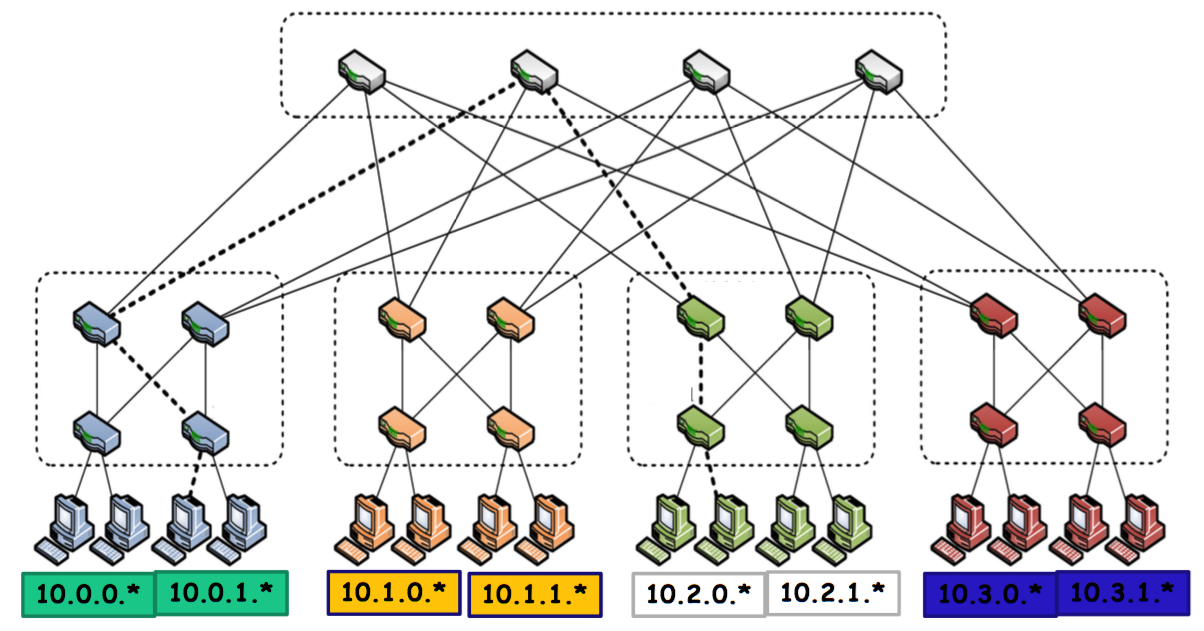
\includegraphics[width=7cm]{fattree}}
\caption{Fattree topology}
\label{fig:fattree}
\end{figure}

\subsection{Controller}

\indent To make SDN MPTCP-aware, it is necessary to let controller know that multipath communication occurs in the network. This can be achieved by packet inspection on controller. When a packet arrives on a forwarder and no rule is matched, the packet is sent to SDN controller which calculates the path for the subflow by using its global view of the topology. SDN controller then installs the rules onto every single forwarder that lies on the chosen path. The implementation will use Floodlight controller written in Java.

\indent The shortest paths available will be computed using a graph traversal algorithm. Sets of paths will be stored on controller and these will be deterministically assigned to subflows. While using multiple redundant paths, MPTCP�s performance should be maximized using a small number of subflows. Each path should be assigned to only one subflow, this can be achieved by storing IP addresses to paths.

\indent When a new packet arrives on the controller, it will extract the needed information from the packet (IPs, ports, MPTCP options). If the option says we are dealing with a new subflow (MP\_CAPABLE), it will find the shortest path between IPs and store the path into a hashtable. This path is then assigned to a subflow. If the options says we are dealing with additional subflow (M \_JOIN), we extract the token from the packet and find another shortest path for the subflow. The rules are installed on all switches belonging to the chosen path.

\subsection{Testbed}
\indent To properly evaluate the algorithm, a virtual testbed will be needed. The tests will be performed on a Linux virtual machine running Floodlight controller and Mininet emulator. We create two more Linux virtual machines with multiple interfaces that will be connected to ports on the switches emulated in Mininet. After running FatTree topology in Mininet, we will evaluate how many subflows are needed in order to maximize MPTCP performance. We will then compare this approach to random approach used by ECMP protocol. 


% Start of "Sample References" section

\section{Typical references in new ACM Reference Format}
A paginated journal article \cite{Abril07}, an enumerated
journal article \cite{Cohen07}, a reference to an entire issue \cite{JCohen96},
a monograph (whole book) \cite{Kosiur01}, a monograph/whole book in a series (see 2a in spec. document)
\cite{Harel79}, a divisible-book such as an anthology or compilation \cite{Editor00}
followed by the same example, however we only output the series if the volume number is given
\cite{Editor00a} (so Editor00a's series should NOT be present since it has no vol. no.),
a chapter in a divisible book \cite{Spector90}, a chapter in a divisible book
in a series \cite{Douglass98}, a multi-volume work as book \cite{Knuth97},
an article in a proceedings (of a conference, symposium, workshop for example)
(paginated proceedings article) \cite{Andler79}, a proceedings article
with all possible elements \cite{Smith10}, an example of an enumerated
proceedings article \cite{VanGundy07},
an informally published work \cite{Harel78}, a doctoral dissertation \cite{Clarkson85},
a master's thesis: \cite{anisi03}, an online document / world wide web resource \cite{Thornburg01}, \cite{Ablamowicz07},
\cite{Poker06}, a video game (Case 1) \cite{Obama08} and (Case 2) \cite{Novak03}
and \cite{Lee05} and (Case 3) a patent \cite{JoeScientist001},
work accepted for publication \cite{rous08}, 'YYYYb'-test for prolific author
\cite{SaeediMEJ10} and \cite{SaeediJETC10}. Other cites might contain
'duplicate' DOI and URLs (some SIAM articles) \cite{Kirschmer:2010:AEI:1958016.1958018}.
Boris / Barbara Beeton: multi-volume works as books
\cite{MR781536} and \cite{MR781537}.

\appendix

\section{Classical Multidimensional Scaling}
\label{sec:cmds}

Let $\mathrm{D}$ be an $n\times n$ matrix of pairwise distances. The
matrix $D$ is symmetric with a zero diagonal. We are interested in
finding a $d \times n$ matrix $\mathrm{X}$ where each column
$\bm{x}_{i}$ is the representation of the point $i$ in $R^{d}$ and
$\mathrm{D}_{ij} = \|\bm{x}_{i}-\bm{x}_{j}\|_{2}$. Denote the inner
product (or Gram matrix) for this set of points by $\mathrm{K} =
\mathrm{X}^{\top}\mathrm{X}$.


$\mathrm{K}$ is an $n\times n$ symmetric positive semidefinite matrix.
Let us now abuse notation and use $\mathrm{D}^{2}$ to indicate the
matrix of squared pairwise distances $\mathrm{K} =
-\frac{1}{2}(\mathrm{I} -
\mathrm{1}\mathrm{1}^{\top})\mathrm{D}^{2}(\mathrm{I} -
\mathrm{1}\mathrm{1}^{\top})$. Here, $\mathrm{I}$ is the $n \times n$
identity matrix and $\mathrm{1}$ is the $n$-vector of all ones.

\begin{acks}
We are grateful to the following people for resources, discussions and
suggestions: Prof. Jacobo Melamed Cattan (Ophthalmology-UFRGS), Prof.
Roberto da Silva (UFRGS), Prof. Luis A. V. Carvalho (Optics-USP/SC),
Prof. Anatolio Laschuk (UFRGS), Leandro Fernandes, Marcos
Slomp, Leandro Lichtenfelz, Renato Silveira,
Eduardo Gastal, and Denison Tavares. We also thank the volunteers who
allowed us to collect pictures and videos of their irises: Alex Gimenes,
Boris Starov, Christian Pagot, Claudio Menezes, Giovane Kuhn, Jo\~{a}o
Paulo Gois, Leonardo Schmitz, Rodrigo Mendes, and Tiago Etiene.
\end{acks}

% Bibliography
\bibliographystyle{ACM-Reference-Format-Journals}
\bibliography{acmtog-sample-bibfile}
                                % Sample .bib file with references that match those in
                                % the 'Specifications Document (V1.5)' as well containing
                                % 'legacy' bibs and bibs with 'alternate codings'.
                                % Gerry Murray - March 2012

\received{September 2008}{March 2009}

\end{document}
% End of v2-acmtog-sample.tex (March 2012) - Gerry Murray, ACM
